\begin{frame}
  \frametitle{Homogenization and Equivalence Theory}
  %
  \begin{block}{} \begin{flushright}
  \textcolor{ceared1}{\Large What for?} Prepare \emph{in advance} all reactor data for later core calculations in \textcolor{ceablue1}{low-order transport} (diffusion, $SP_N$ and others). \end{flushright}
  \end{block}\vspace{5mm}
  %
  \begin{alertblock}{Main rational of Homogenization}
    Conservation of reaction rates in the volume $\mathcal{V}$ of
    \emph{spatial homogenization} and
    in the $g$-th group of \emph{energy condensation} with
    $E \in [E_g, E_{g+1}]$, $g = 1, \ldots, G$.
  \end{alertblock}
  %
  \[
  \Sigma_g = \frac{\displaystyle
    \int_{\mathcal{V}} d\mathbf{r} \int_{E_{g+1}}^{E_g} dE \,
      \Sigma(\mathbf{r}, E) \, \phi(\mathbf{r}, E) }{\displaystyle
    \int_{\mathcal{V}} d\mathbf{r} \int_{E_{g+1}}^{E_g} dE \, \phi(\mathbf{r}, E)
    } \quad \text{with} \quad \chi_g = \int_{E_{g+1}}^{E_g} dE \, \chi(E).
  \]
  %
  \begin{columns}
    \column{.6\textwidth}
      \begin{block}{Equivalence}
      \textcolor{ceared1}{\Large Why?} $\ldots$Diffusion $\not\equiv$ transport, conservation of reaction rates does not imply to reproduce the \emph{same currents} at the boundaries of $\mathcal{V}$. Available techniques:
      \begin{itemize}
        \item (A)DF$ = \phi_{\text{het}}/\phi_{\text{hom}} $ (discontinuity factors), \emph{two per direction}
        \item SPH (SuPer-Homogenization) factors, \emph{one per group and homog. region}: $(\Sigma^{(k)}_g / s)(s\phi^{(k)}_g)$
      \end{itemize}
    \end{block}
    %
    \column{.4\textwidth} \centering
    \def\wdt{2.5}
    \def\ymin{0.25}
    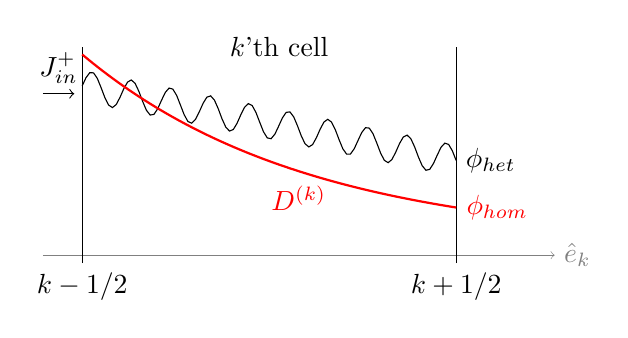
\begin{tikzpicture}
      \draw[->, thin, help lines] ({-\wdt-0.5},{\ymin+0.1})
        -- ({\wdt+1},{\ymin+0.1}) node[right] {$\hat{e}_k$};
      \draw[-] (-\wdt,\ymin) node[below] {$k-1/2$} -- (-\wdt,3);
      \draw[-] ({\wdt-1/4},\ymin) node[below] {$k+1/2$} -- ({\wdt-1/4},3);
      \draw[->] ({-\wdt-0.5}, 2.4) -- ({-\wdt-0.1}, 2.4)
        node[midway,above] {$J^+_{\text{in}}$};
      \draw[black, domain={-\wdt}:{\wdt-1/4}]
        plot[samples=100]
        ({\x}, {2+0.2*sin(((\x+2)*4)*3.141592 r)-0.2*\x})
        node[right] {$\phi_{\text{het}}$};
      \draw[red, domain={-\wdt}:{\wdt-1/4}, thick]
        plot[samples=100] ({\x}, {0.5+exp(-0.35*\x)})
        node[right] {$\phi_{\text{hom}}$};
      \node[red,below] (D) at (\ymin,1.35) {$D^{(k)}$};
      \node (title) at (0,3) {$k$'th cell};
    \end{tikzpicture}
  \end{columns}
\end{frame}
